\documentclass[12pt,a4paper]{article} 
\usepackage[russian]{babel} 
\usepackage[utf8]{inputenc}
\usepackage[left=3cm,right=3cm,top=3cm,bottom=3cm]{geometry} 
\usepackage{tikz} 
\usepackage{amsfonts} 
\usepackage{amsthm} 
\usepackage{amsmath} 
\usepackage{amssymb} 
\usepackage{moreverb} 
\usepackage{hyperref} 
\usetikzlibrary{calc,intersections} 
\usepackage{graphics} 
\usepackage{multirow} 
\graphicspath{{image/}} 
\sloppy 

\theoremstyle{definition} 
\newtheorem{mydef}{Определение}[section] 
\begin{document} 

\begin{titlepage} 
\newpage % НАЧАЛО ТИТУЛЬНОГО ЛИСТА 
\begin{center} 
\begin{figure}[h] 
	\center 
	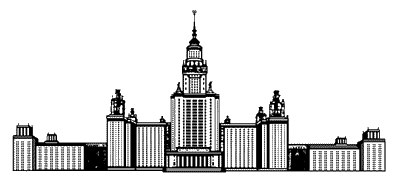
\includegraphics[scale=0.4]{msu2.jpg} 
\end{figure} 
\footnotesize {Московский государственный университет} 
\footnotesize {имени М. В. Ломоносова} 
\linebreak 
\normalsize {Факультет вычислительной математики и кибернетики} 
\linebreak 
\normalsize {Кафедра математических методов прогнозирования} 
\linebreak 
\linebreak 
\linebreak 
\large{\text {Трубицын Юрий Алексеевич}} 
\linebreak 
\linebreak 
\large{\textbf{Распознавание последовательности числительных дактильной азбуки}} 
\linebreak 
\linebreak 
\large{\text {КУРСОВАЯ РАБОТА}} 
\linebreak 
\linebreak 
\end{center} 
\begin{flushright} 
\Large {\bf Научный руководитель:}\\ 
\Large д. т. н., профессор\\ 
\Large Л. М. Местецкий\\ 
\end{flushright} 
\vspace{\fill} 
\begin{center} 
\large{Москва, 2018} 
\end{center} %\thispagestyle{empty} 
\end{titlepage} 
\newpage 
\pagestyle{plain} 
\tableofcontents 

\newpage 
\section{\textbf{Введение}} 
В данной работе предметом исследования является азбука глухонемых, или \textbf{дактильная азбука} (также известная как \textbf{дактилология}). Под дактильной азбукой понимается вспомогательная система жестового языка, в которой каждому жесту одной руки (обычно неподвижной правой, согнутой в локте) соответствует буква языка; многие знаки внешне похожи на соответствующие буквы алфавита.\par 
В данном исследовании под жестом понимается статическая форма и положение кисти правой руки на изображении. Под числительными дактильной азбуки будем понимать жесты, обозначающие десятичные цифры. Задача распознавания последовательности числительных дактильной азбуки состоит в выделении из видеопотока последовальности жестов, обозначающих числительные дактильной азбуки.\par 
Задача распознавания жестов дактильной азбуки достаточно хорошо изучена и существуют алгоритмы, которые хорошо справляются с этой задачей на основе RGB-картинок. Но с ростом технологий появляются	новые виды сенсоров. Помимо обычных веб-камер, появляются новые виды - \textbf{камеры глубины}. Они предоставляют новые возможности для исследований и улучшений уже существующих алгоритмов. В данной работе исcледования проводятся с помощью камеры глубины Intel SR300. Она позволяет получать карту глубины картинок в видеопотоке в онлайн режиме, что позволяет выделять 3D-скелет кисти руки на каждом кадре видеопотока.\par 
Основная задача данной работы заключается в раз­работке метода классификации динамических жестов по видеопоследователь­ности на основе 3D-скелета кисти. В качестве объектов, совершающих жесты, рассматриваются рука и тело человека. Сложность задачи определяется очень большим разнообразием индивидуальных антропометрических и двигательных особенностей различных людей, требованием реального времени работы системы компьютерного зрения.\par 
Распознавание жеста затруднено в связи с неточностями построения 3D-скелета кисти, что приводит к серьезным осложнением в классификации данного жеста. Также, возникает проблема выделения последовательности цифр из динамического видеоряда жестов, которые являются различными по продолжительности и могут повторяться.\par 
В данной работе предлагается подход к классификации жестов на основе состояния пальцев кисти, а также эвристический способ выделения последовательности цифр из видеоряда в режиме онлайн. 
\noindent 

\newpage 
\section{Постановка задачи} 
Были поставлены следующие задачи:
\begin{enumerate}
\item Классификация жестов числительных дактильной азбуки на основе 3D-скелета кисти;
\item Выделение последовательности цифр из видеопотока жестов на основе результатов покадровой классификации;
\end{enumerate}

\newpage
\section{Основная часть}
\subsection{Классификация жестов числительных дактильной азбуки на основе 3D-скелета кисти}
Основным результатом данной работы является алгоритм выделения последовательности цифр из видеопотока жестов числительных дактильной азбуки.
\subsubsection{Вход алгоритма}
%Введем ряд определений.

\begin{mydef}
\emph{Метрическим пространством} будем называть пару $\left(\mathcal{F}, \rho_{\mathcal{F}}\right)$, где $\mathcal{F}$ - непустое множество, а $\rho_{\mathcal{F}}$ - отображение $\mathcal{F} \times \mathcal{F}  \rightarrow \mathbb{R}$, называемое метрикой и удовлетворяющее следующим аксиомам:
\begin{itemize}
\item $\rho_{\mathcal{F}}\left(x, y\right) = 0 \Leftrightarrow x = y$,
\item $\rho_{\mathcal{F}}\left(x, y\right) = \rho_{\mathcal{F}}\left(y, x\right)$,
\item $\rho_{\mathcal{F}}\left(x, z\right) \leq \rho_{\mathcal{F}}\left(x, y\right) + \rho_{\mathcal{F}}\left(y, z\right)$,
\end{itemize}
$\forall x, y, z \in \mathcal{F}$
\end{mydef}

\begin{mydef}
\emph{Помеченным пространственным графом} в метрическом пространстве $\left(\mathcal{F}, \rho_{\mathcal{F}}\right)$ на множестве меток $\mathcal{L}$ будем называть граф $G = (V, E)$, в котором:
\begin{enumerate}
\item $V=\left\{\left(v_1, l_1\right), ..., \left(v_n, l_n\right)\right\}, v_i \in \mathcal{F}, l_i \in \mathcal{L}\  \forall i = \overline{1, n}$.
\item $E=\left\{\left(u, v\right)\right\}, u, v \in V$ - множество неупорядоченных пар из $V$.
\end{enumerate}
\end{mydef}

Пронумеруем пальцы одной руки от одного до пяти в порядке от большого пальца к мизинцу. Заметим, что все пальцы у здорового человека, кроме большого, имеют по три фаланги, называемых в анатомии дистальная фаланга, средняя фаланга и проксимальная фаланга. Большой палец имеет только две фаланги: дистальную и проксимальную.
\begin{figure}[h] 
	\center 
	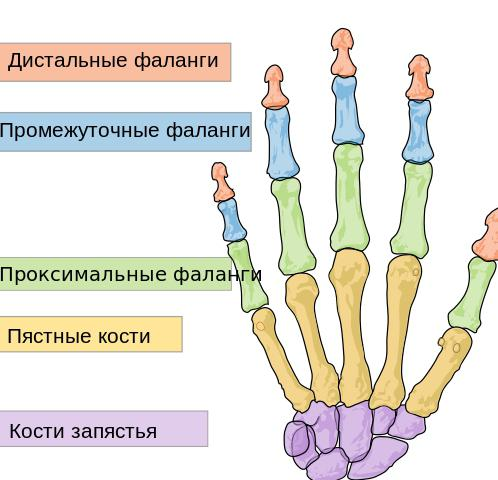
\includegraphics[scale=0.4]{falangs.jpeg} 
\end{figure}

Пронумеруем места стыков пястной кости и проксимальной фаланги, проксимальной и средней фаланги, средней и дистальной фаланги, а также верхний пик дистальной фаланги от одного до четырех соответственно.\par
Тогда мы можем каждый палец представить в виде множества меток $L_i = \left(l_{i1}, l_{i2}, l_{i3}, l_{i4}\right), i = \overline{2, 5}$, где $l_{ij}$ соответствует j-ому месту стыка i-го пальца.\par
В случае большого пальца пронумеруем места стыков пястной кости и проксимальной фаланги, проксимальной и дистальной фаланги, а также верхний пик дистальной фаланги от одного до трех соответственно. Получим множество меток для большого пальца $L_1 = \left(l_{11}, l_{12}, l_{13}\right)$, где $l_{1j}$ соответствует j-ому месту стыка большого пальца

Будем понимать под центром ладони центр окружности максимального радиуса, вписанной в фигуру, образуемую границами ладони. Добавим ещё три метки:
\begin{enumerate}
\item $l_c$ - так называемый центр ладони;
\item $l_w$ - центр фигуры, ограниченной запястными костями;
\item $l_{wc}$ - место стыка пястной кости большого пальца и запястья. 
\end{enumerate}

Таким образом, на вход алгоритма подается 3D-скелет ладони, представленный в виде помеченного пространственного графа $G = (V, E)$ в метрическом пространстве $\left(\mathbb{R}^3, l_2\right)$ на множестве меток $L = \bigcup_{i=1}^5 L_i \cup l_c \cup l_w \cup l_{wc}$, в котором:
\begin{itemize}
\item $V = \left\{{\left\{u_{ij}\right\}}_{i=2,j=1}^{5,4}, {\left\{u_{1j}\right\}}_{j=1}^{3}, u_{c}, u_w, u_{wc}\right\}, u_{ij} = \left(v_{ij}, l_{ij}\right), u_c = \left(v_c, l_c\right), u_w = \left(v_w, l_w\right), u_{wc} = \left(v_{wc}, l_{wc}\right), |V| = |L| = 22$;
\item $E = \left\{ {\left\{\left(u_{ij}, u_{i,j+1}\right)\right\}}_{i=2, j=1}^{5, 3}, {\left\{\left(u_{1j}, u_{1,j+1}\right)\right\}}_{j=1}^{2}, {\left\{\left(u_w, u_{i1}\right)\right\}}_{i = 2}^{5}, \left(u_w, u_{wc}\right), \left(u_{wc}, u_{11}\right) \right\}$
\end{itemize}

\begin{figure}[h] 
	\center 
	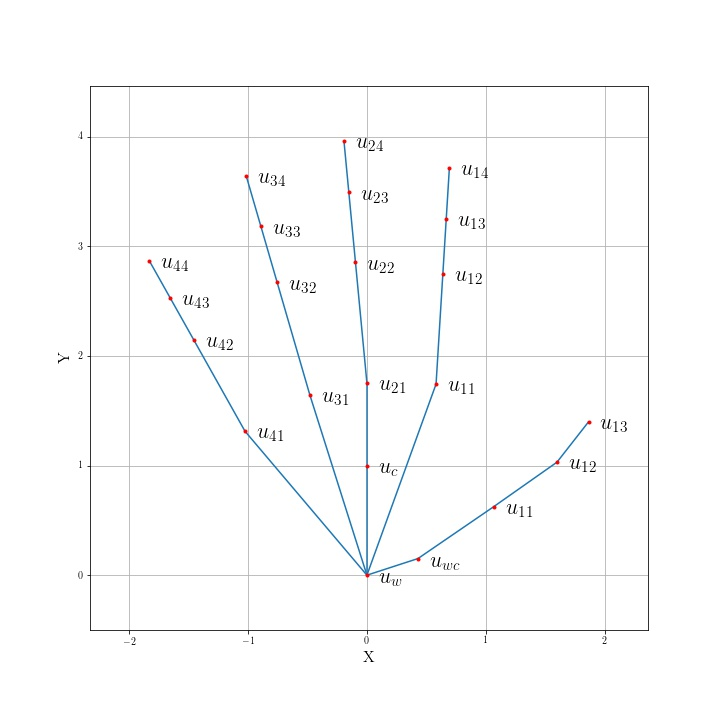
\includegraphics[scale=0.35]{hand.jpeg} 
\end{figure}





\end{document} 